\documentclass[11pt]{article}
\usepackage[utf8]{inputenc}

\usepackage{graphicx}
\usepackage[left=0.8in,right=1.0in,top=1.0in,bottom=1.0in]{geometry}
\usepackage [english]{babel}
\usepackage [autostyle, english = american]{csquotes}
\MakeOuterQuote{"}
\usepackage{caption}
\usepackage{subcaption}

\addto\captionsenglish{\renewcommand*\contentsname{Table of Contents}}


\title{Indeed Product Science Homework}


\begin{document}

\maketitle

\newpage

\tableofcontents

\newpage



\section{Nomenclature}
\begin{enumerate}
    \item The terms "Customer","Lead", and "Advertiser" all refer to sales leads.
    \item The terms "Field" and "Column" both refer to the set of values stored in a specific column in the data-set provided, including new columns added to the data-set (see Data-Set Transformations).
    \item An "Assigned Lead" refers to a lead that has been assigned to a sales representative. They appear in the data-set by having a "1" value in the "assigned" column.
     \item An "Unassigned Lead" refers to a lead that has never been assigned to a sales representative. They appear in the data-set by having a "0" value in the "assigned" column.
    \item Any further discussion on revenue will be referring to the values attained from the transformed "Cleaned Revenue" column, and not the original "revenue" column. See "Data-Set Transformations" for more details.
    \item A customer is a "Revenue Generating Customer", or is said to have "generated revenue" if their corresponding entry in the "Cleaned Revenue" column is a positive non-zero number.
\end{enumerate}
\section{Data-set Assumptions}
\begin{enumerate}
    \item Each unique value in the "advertiser\_id" column represents an identification number for a unique customer.
    \item The "revenue" column represents revenue generated by an advertiser, and the units of the field are \$USD in thousands of cents, (or ten-thousandths of a dollar).
    \item Any customer that has a valid date in the column "first\_revenue\_date" but has no entry in the "revenue" column indicates that the customer at one point has generated revenue, but has not generated revenue since being assigned to a sales lead. 
    \item Furthermore, any customer who's "revenue" column is null indicates that the customer has not generated revenue since being added to the data-set. 
    \item Customers should be bifurcated on whether or not they have been assigned to a sales representative, and on whether or not they have generated revenue.
    \item \textbf{In this analysis it is assumed that the data-set provided is a representative sample of a larger population of assigned and unassigned sales leads.} 
\end{enumerate}

\section{Data-set Transformations}
\begin{enumerate}
    \item The "Cleaned Revenue" column is defined by scaling the values of the "revenue" column by $\frac{1}{10000}$. If the "revenue" column is null, then the value is set to 0. The units of this column are \$USD.
    \item The "Age in Years" column is defined by scaling the values in the "age" column by $\frac{1}{365}$.
\end{enumerate}

\newpage

\section{Question 1}

There are $77,891$ sales leads within the data-set, with $37,079$ ($47\%$) leads assigned to sales representatives, and $40,812$ ($53\%$) leads not assigned to sales representatives. 
\par Of the $37,079$  assigned leads, $1,565$ ($4.2\%$) had revenue recorded in the data-set. The assigned leads generated $\$12M$ in revenue, or $73.9\%$ of total revenue recorded in the data-set for all leads. For the total sample of assigned leads, the average revenue was $\$323.88$ per lead, but, when only considering the assigned leads that generated revenue, the average revenue per lead was $\$7,673.69$. The average age of all assigned leads is 638 days, and when only considering revenue generating assigned leads, the average age falls to 473 days.

Of the $40,812$ unassigned leads, $1,775$ ($4.4\%$) have revenue recorded in the data-set. The unassigned leads totaled $\$4.2M$ in revenue, or $26.1\%$ of total lead revenue. For the total sample of unassigned leads the average revenue was $\$103.90$, and when considering only the unassigned leads that generated revenue, the average revenue per lead was $\$2,388.94$. The average age of all the unassigned leads is 12 days, and when only considering revenue generating unassigned leads, the average age increases to 23 days. \\

\textbf{Observations:}
\begin{itemize}
    \item When comparing customers that were assigned sales leads to those that were not, \textbf{on average, the revenue generated by a lead assigned to a sales representative is \textit{three times} that of a lead that was not assigned}, regardless if we consider the total sample of each group or only the revenue generating members of each group. 
    \item The percentage of leads that generated revenue is nearly identical for both unassigned leads ($4.4\%$) and assigned leads ($4.2\%$).
    \item $95\%$ ($1,682$ of $1,775$) of the revenue-generating unassigned leads have a "date\_created" value in the range 02-01-2017 to 02-04-2017. This seems highly suspicious, and could indicate an error within our data. \textbf{This could potentially complicate understanding the relationship between lead age and revenue.} 
\end{itemize}

\begin{center}
\begin{table}[h]
    \centering
    \begin{tabular}{|c|c|c|}
    \hline
     \textbf{Sample} & \textbf{Customer Count} & \textbf{Average Revenue}\\ 
     Assigned & 37,079  & \$323.88 \\
     Unassigned & 40,812 &\$103.90 \\
     Total & 77,891 & \$208.62 \\ 
     \hline 
\end{tabular}
    \caption{Average Revenue by Sample, All Customers}
\end{table}
\end{center}
\begin{center}
\begin{table}[h!]
    \centering
    \begin{tabular}{|c|c|c|}
    \hline
     \textbf{Sample} & \textbf{Customer Count} & \textbf{Average Revenue}\\ 
     Assigned & 1,565  & \$7,673.69 \\
     Unassigned & 1,175 & \$2,388.94 \\
     Total & 3,340 & \$4,865.18 \\
     \hline 
\end{tabular}
    \caption{Average Revenue by Sample, Revenue-Generating Customers Only}
\end{table}
\end{center}

\newpage 

\begin{figure}[h!]
    \centering
    \begin{subfigure}[l]{0.45\textwidth}
         \centering
        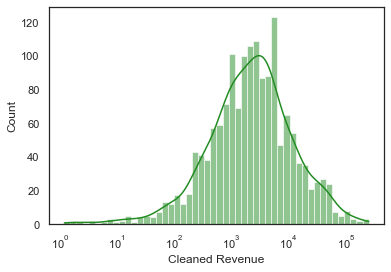
\includegraphics[scale=.5]{Images/Assigned_Revenue_Histogram.png}
         \caption{Revenue Distribution \mu=7,674 \  \sigma=18,637}
         \label{fig:revenue distribution}
     \end{subfigure}
       \begin{subfigure}[r]{0.4\textwidth}
         \centering
       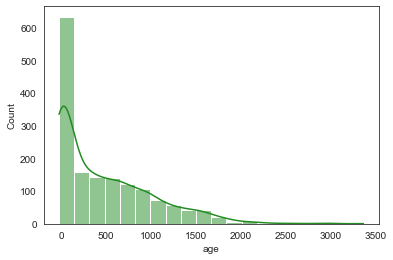
\includegraphics[scale=.5]{Images/assigned_date_created_histogram.png}
         \caption{Age distribution \mu=473 \ \sigma=529}
         \label{fig:date distriburtion}
     \end{subfigure}
    \caption{Distributions for Revenue-Generating Assigned Leads (Count = 1,565)}
    \label{fig:assigned_lead_rev}
\end{figure}


\begin{figure}[h!]
    \centering
    \begin{subfigure}[l]{0.45\textwidth}
         \centering
        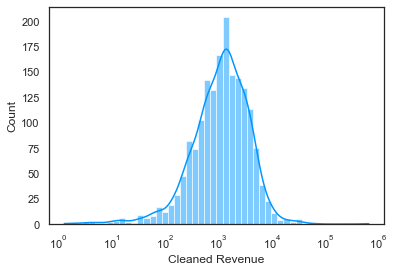
\includegraphics[scale=.5]{Images/Unassigned_Revenue_Histogram.png}
         \caption{Revenue Distribution, \mu = 2,389 \ \sigma = 15,764}
         \label{fig:revenue distribution}
     \end{subfigure}
       \begin{subfigure}[r]{0.4\textwidth}
         \centering
       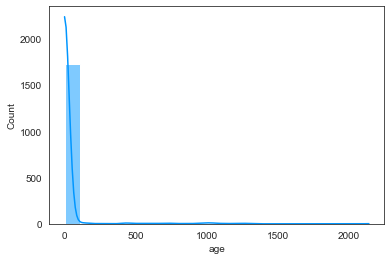
\includegraphics[scale=.5]{Images/unassigned_date_created_histogram.png}
         \caption{Age distribution \mu=23 \ \sigma=145}
         \label{fig:date distriburtion}
     \end{subfigure}
    \caption{Distribution for Revenue-Generating Unassigned Leads (Count = 1,775)}
    \label{fig:assigned_lead_rev}
\end{figure}


\begin{table}[h]
    \centering
    \scalebox{0.85}{
    \begin{tabular}{|c|c|c|c|c|c|c|c|}
        \hline 
         \textbf{Sample} & \textbf{Count}&\textbf{Revenue, Sum} & \textbf{Revenue, Avg} &  \textbf{\% of Total Revenue }& \textbf{Std. Dev. Revenue}& \textbf{Avg Age (Days)}\\
         Assigned & 1565 & \$12,009,319 & \$7,674 &  74\% & \$18,636 & 473\\
         Unassigned & 1775 & \$4,240,371 & \$2,389 &  26\% & \$15,764 & 23\\
         Total & 3340 & \$16,249,690 & \$4,865 &  100\% & \$17,368 & 234\\
         \hline
    \end{tabular}}
    \caption{Descriptive Statistics for Revenue-Generating Leads}
    \label{tab:my_label}
\end{table}         


\newpage

\section{Question 2}
\textit{What are the most important metrics to consider when answering the problem
statement? Why?} \\

Some of the most important metrics to consider when answering the problem statement are actually missing from our data. \\

In the "Background" section of the problem statement, it is explained that Indeed routes leads to the sales team based on the quality of each lead, credit to some system that predicts potential dollar value and probability of success for each lead. To answer the question posed in the problem statement, "How much more did leads spend because there was a sales intervention", it is vital to understand the probability and value assigned to each lead, for both unassigned and assigned leads alike. \\

Without this additional data, if we compare the assigned and unassigned leads blindly, we risk making an unfair comparison, that is to say, we could be comparing apples to oranges. Lets say we analyze our data as is, and we conclude that thanks to our sales interventions we extract more revenue out of each lead by virtue of our highly skilled sales personnel. In reality, it is very likely that we are comparing low dollar value leads that our system did not assign, to high dollar value leads our system assigned to our sales personnel, (hence the apples to oranges comparison). The differences we note in revenue would be valid, though the conclusions regarding our sales personnel spurious. If we decide to use this information to expand our sales team in order to grow revenues, in reality we would be increasing costs while not necessarily augmenting revenue. \\

However, if we have the estimated dollar values and probabilities that our system assigns to our leads in our data, we can employ a much more rigorous approach by comparing like samples of assigned leads and unassigned leads directly, (apples to apples at last). For example, we could analyze the revenue generated from low-dollar, low-probability leads that were assigned to our sales team, and compare the sample with low-dollar, low-probability leads that were not assigned. If we note a difference between the samples (a statistically significant difference at that) we can draw conclusions regarding the efficacy of our sales team in a much more legitimate way.  \\

Furthermore, any additional data on our customers would help us with understanding the efficacy of our sales team dramatically. For instance, if we could add fields to our data-set that describe the industry, company size (in revenue dollars and market capitalization), and location of our sales leads, we would be able to more comprehensively understand our lead demographics. For example, companies in different industries or locations may have different advertisement strategies, and companies of varying size will have different marketing budgets. In any case, our customers will have different advertising needs and resources to allocate to our services, and thus will generate different revenues. With more granular data we will be able to accurately segment and compare like customers to fully understand the impact our sales interventions have on revenue. \\

In short, we are missing fields in our data-set that would allow us to create meaningful comparisons between our customer demographics. With additional information we would be able to understand the relationship between sales interventions and revenue in a much more rigorous and clear manner.

\newpage

\section{Question 3}
\textit{Analyze any existing relationship between account age and revenue} \\

Overall, it is difficult to understand the relationship between account age and revenue for two main reasons. Firstly, for unassigned leads, $95\%$ of the leads that generated revenue have an account age between 0 and 3 days. This distribution of age data points is highly suspicious, and could be indicative of an error within our data. As a result, unassigned leads may not be useful in understanding the relationship between account age and revenue. Secondly, in both the assigned and unassigned leads there are many outliers which obscure the relationship we are trying to observe. 

Consider the following two scatterplots between age and revenue for both samples of revenue-generating leads. Note how for each distribution there is not a strong relationship between the two axes, illustrated by the very low values of each Pearson correlation coefficient ($\rho$). \\

\begin{figure}[h]
    \centering
    \begin{subfigure}[l]{0.45\textwidth}
         \centering
        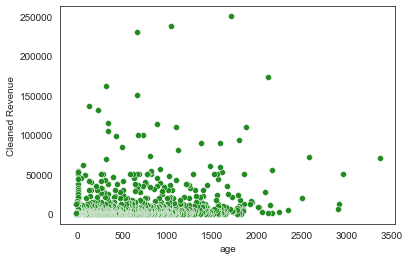
\includegraphics[scale=.5]{Images/assigned_scatter_age_vs_cleaned_revenue.png}
         \caption{Assigned Leads, $\rho = 0.200$}
         \label{fig:revenue distribution}
     \end{subfigure}
       \begin{subfigure}[r]{0.4\textwidth}
         \centering
       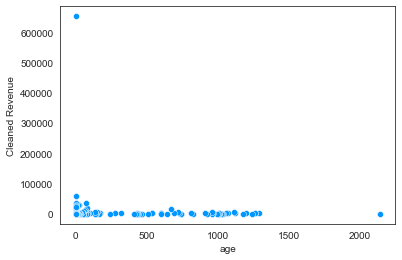
\includegraphics[scale=.5]{Images/unassigned_scatter_age_vs_cleaned_revenue.png}
         \caption{Unassigned Leads, $\rho = -0.001$}
         \label{fig:date distriburtion}
     \end{subfigure}
    \caption{Scatter-plots for Revenue-Generating Leads, Cleaned Revenue by Age}
    \label{fig:assigned_lead_rev}
\end{figure}

We can further investigate if there is a relationship between age and revenue, by performing a linear regression on account age in years (\textbf{binned by half-years}) against the \textbf{average revenue of each half-year}. Doing so yields the following plots:

\begin{figure}[h]
    \centering
    \begin{subfigure}[l]{0.45\textwidth}
         \centering
        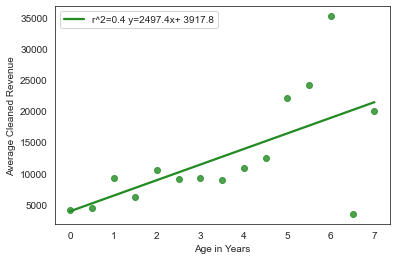
\includegraphics[scale=.5]{Images/assigned_regplot.png}
         \caption{Assigned Leads, $r^2=0.4$}
         \label{fig:revenue distribution}
     \end{subfigure}
       \begin{subfigure}[r]{0.4\textwidth}
         \centering
       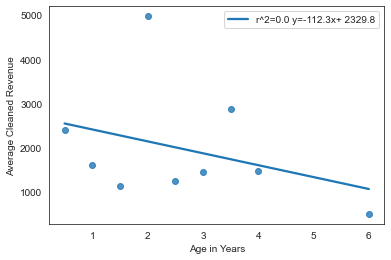
\includegraphics[scale=.5]{Images/Unassigned_regplot.png}
         \caption{Unassigned Leads, $r^2=0.0$}
         \label{fig:date distriburtion}
     \end{subfigure}
    \caption{Regression-Plots for Revenue-Generating Leads, Cleaned Revenue by Age in Years}
    \label{fig:assigned_lead_rev}
\end{figure}

\newpage 

\begin{table}[h]
    \begin{subtable}[h]{0.45\textwidth}
        \centering
         \begin{tabular}{c|c|c}
        \textbf{Age in Years} & \textbf{Mean} & \textbf{Count} \\
        \hline
        0 - 0.5 & \$4,414 & 649 \\
        0.5 - 1 &\$9,272 & 177 \\
        1 - 1.5 &\$6,151 & 144 \\
        1.5 - 2 &\$10,477 & 152 \\
        2 - 2.5 &\$9,129 & 110 \\
        2.5 - 3 &\$9,195 & 110 \\
        3 - 3.5 &\$8,957 & 61 \\
        3.5 - 4 &\$10,799 & 50 \\
        4 - 4.5 &\$12,456 & 45 \\
        4.5 - 5 &\$22,087 & 24 \\
        5 - 5.5 &\$24,102 & 10 \\
        5.5 - 6 &\$35,171 & 8 \\
        6 - 6.5 &\$3,491 & 2 \\
        6.5 - 7 &\$20,000 & 1 \\
        \end{tabular}
       \caption{Revenue-generating Assigned Leads}
       \label{tab:week1}
    \end{subtable}
    \hfill
    \begin{subtable}[h]{0.45\textwidth}
        \centering
        \begin{tabular}{c|c|c}
    \textbf{Age in Years} & \textbf{Mean} & \textbf{Count} \\
    \hline
        0 - 0.5 &\$2,397 & 1728 \\
        0.5 - 1 &\$1,610 & 3 \\
        1 - 1.5 &\$1,122& 10 \\
        1.5 - 2 &\$4,971& 7 \\
        2 - 2.5 &\$1,242& 5 \\
        2.5 - 3 &\$1,455& 13 \\
        3 - 3.5 &\$2,873& 7 \\
        3.5 - 4 &\$1,475 & 1 \\
        4 - 4.5 & nan & 0 \\
        4.5 - 5 & nan & 0 \\
        5 - 5.5 & nan & 0 \\
        5.5 - 6 &\$498 & 1 \\
        6 - 6.5 & nan & 0 \\
        6.5 - 7 & nan & 0 \\
        \end{tabular}
    \caption{Revenue-generating Unassigned Leads}
        \label{tab:week2}
     \end{subtable}
     \caption{Average Revenue Per Age in Years, Revenue-Generating Leads Only}
     \label{tab:Table 3}
\end{table}

Again, the relationship between average revenue and age in years is not explained well by a linear model, hence the low $r^2$ value for the assigned sample, and the non-existent $r^2$ value for the unassigned sample. However, if we only consider the assigned sample, it is fair to say that \textbf{on average as account age in years increases, the average revenue generated \textit{generally} increases as well.} We can see this illustrated in Table 3 (a) above, and the relationship seems to hold for the first 5 years, (beyond 5 years, there are too few samples for the average revenue to be meaningful). If we only consider the first five years, there is a moderate positive correlation between account age in years and average revenue ($r^2=0.7$). 

\begin{figure}[h!]
    \centering
    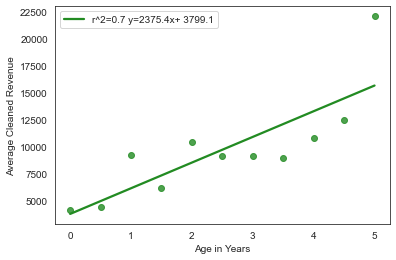
\includegraphics[scale=.5]{Images/assigned_regplot_5years.png}
    \caption{Revenue-Generating Assigned Leads, Account Age 0-5 Years, $r^2=0.7$}
    \label{fig:my_label}
\end{figure}

In conclusion, \textbf{it is difficult to define a meaningful relationship between account age and revenue,} due to the significant variance in the revenue generated by each group of leads, and the questionable age data for unassigned leads. \textbf{In general, as the account age increases for assigned leads, so does the average revenue.} This conjecture intuitively make sense, as larger leads are more likely to have more sophisticated advertising needs, and therefore the sales process would take longer to close for customers that would generate more revenue.








\newpage

\section{Question 4}\\
For the reasons stated in my Question 2 response, we currently do not have enough data to answer this question without making large (and certainly incorrect) assumptions. To reiterate: if we want to accurately answer this question, we will need to have the estimated dollar value and assigned probability generated by our internal system for each of the advertisers in our data-set. With the additional data, we could compare like samples from each group to understand the effect of our sales interventions. Without this information, we must make assumptions to justify comparing the two customer groups. \\

If we assume that the assigned and unassigned groups are virtually identical, with the only difference between groups being whether or not they were assigned to a sales representative, we can begin to analyze the impact of our sales interventions. On average each unassigned lead generates $\$2,388$ in revenue, but if we assign the lead to a sales representative, the revenue generated increases to $\$7,673$. This means each sales intervention increases the revenue generated by $221\%$, or $\$5,285$ dollars per lead.

\begin{center}
\begin{table}[h]
    \centering
    \scalebox{0.9}{
    \begin{tabular}{|c|c|c|}
    \hline
     \textbf{Sample} & \textbf{Customer Count} & \textbf{Average Revenue}\\ 
     Assigned & 1,565  & \$7,673.69 \\
     Unassigned & 1,175 & \$2,388.94 \\
     Total & 3,340 & \$4,865.18 \\
     \hline 
\end{tabular}}
    \caption{Average Revenue by Sample, Revenue-Generating Customers Only}
\end{table}
\end{center}

\begin{figure}[b!]
    \centering
    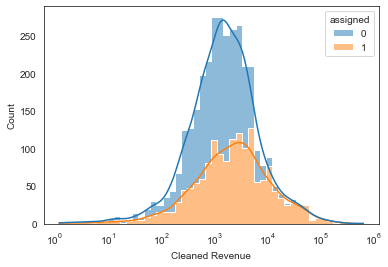
\includegraphics[scale=.5]{Images/joint_histogram.png}
    \caption{Revenue Distributions of Assigned and Unassigned Samples}
    \label{fig:my_label}
\end{figure}
We can perform an Independent T-Test to verify that the differences we observe between the two samples is statistically significant. The Independent T-Test is a great statistical test for our current circumstances: we do not know our true population parameters (we only have the samples in the data-set), and we can assume the variance between assigned and unassigned leads is the same. For our null hypothesis, we hold that having a sales intervention has no effect on revenue. We set a significance level of $\alpha=0.05$, and we perform our Independent T-Test. What we get is a test statistic of $8.87$ and a p-value of $1.10 \times e^-18$, much smaller than our significance level. We can conclude that the differences in our sample means are not attributable to chance alone, and we decide to reject the null hypothesis that the sample means of unassigned and assigned leads are the same. We decide to conclude that our sales intervention had an effect, and that \textbf{on average, for each lead we assign, we generate $321\%$ of the revenue we normally would, an increase of $\$5,285$ per lead.}  


\newpage


\section{Question 5}
\textit{Investigate the data however you wish and discuss any interesting insights you
can find in the data. Don't feel pressured to spend hours on this.}\\

\textbf{Observations:}
\begin{itemize}
    \item When comparing customers that were assigned sales leads to those that were not, \textbf{on average, the revenue generated by a lead assigned to a sales representative is \textit{three times} that of a lead that was not assigned}, regardless if we consider the total sample of each group or only the revenue generating members of each group. 
    \item The percentage of leads that generated revenue is nearly identical for both unassigned leads ($4.4\%$) and assigned leads ($4.2\%$).
    \item $95\%$ ($1,682$ of $1,775$) of the revenue-generating unassigned leads have a "date\_created" value in the range 02-01-2017 to 02-04-2017. This seems highly suspicious, and could indicate an error within our data. \textbf{This could potentially complicate understanding the relationship between lead age and revenue.} 
    \item There are 5,093 data points that have a date recorded for the "first\_revenue\_date" column, but no revenue recorded in the data-set
\end{itemize}



\end{document}
